\chapter{Radio Frequency Interference (RFI) and Site Testing}

\section{Overview}

One of the challenges of radio astronomy is locating sites that meet the environmental and atmospheric requirements of a particular set of observations. Potential sites must be assessed for their viability prior to significant experiment development and observation at those sites. Site assessment must include four elements, each of which must be addressed to evaluate the site quality. 

First, does the site have any nearby man-made sources of regular radio frequency interference (RFI) in the frequency band of the observations. Evaluation of this requirement can be done using a simple broadband antenna and spectrum analyzer on site at multiple locations. Deployment of an identical system at different sites allows a much more reliable comparison than can be made with independent systems. 

Second, is the site logistically accessible for the type of equipment needed for a set of observations. Some important considerations include the availability of power, transport into/out of the location, housing and other observer requirements and site access permissions (such as permits). Assessment of these considerations often requires an in-person visit and careful documentation. 

Third, are there atmospheric effects that must be considered in assessing the viability of a site (eg meteor scatter, thickness of ionosphere, inclement weather). Tracking data may be available from external sources such weather surveys, but it is often limited to broad trends instead of local details. 

Fourth, are there sources of intermittent or highly time-variable RFI visible from the site. This can be more difficult to evaluate as it requires a long period of data collection. In cases where time-variable RFI is expected to play a significant role in the data collection, semi-permanent systems may need to be installed to track the RFI environment over time. 

In the following sections, I am going to evaluate both existing telescope sites and new sites based upon the requirements listed above. I will set a baseline using Pittsburgh, Pennsylvania; which as a major metropolitan area is not expected to be a suitable radio astronomy site. I will then look at several existing radio telescope sites and examine their strengths and weaknesses. Finally, I will report on several new radio sites, comparing them to the existing sites to demonstrate viability. 

\subsection{Site Testing Kit}

\begin{figure}[htb]
\centering
\begin{minipage}[b]{0.47\textwidth}
\centering
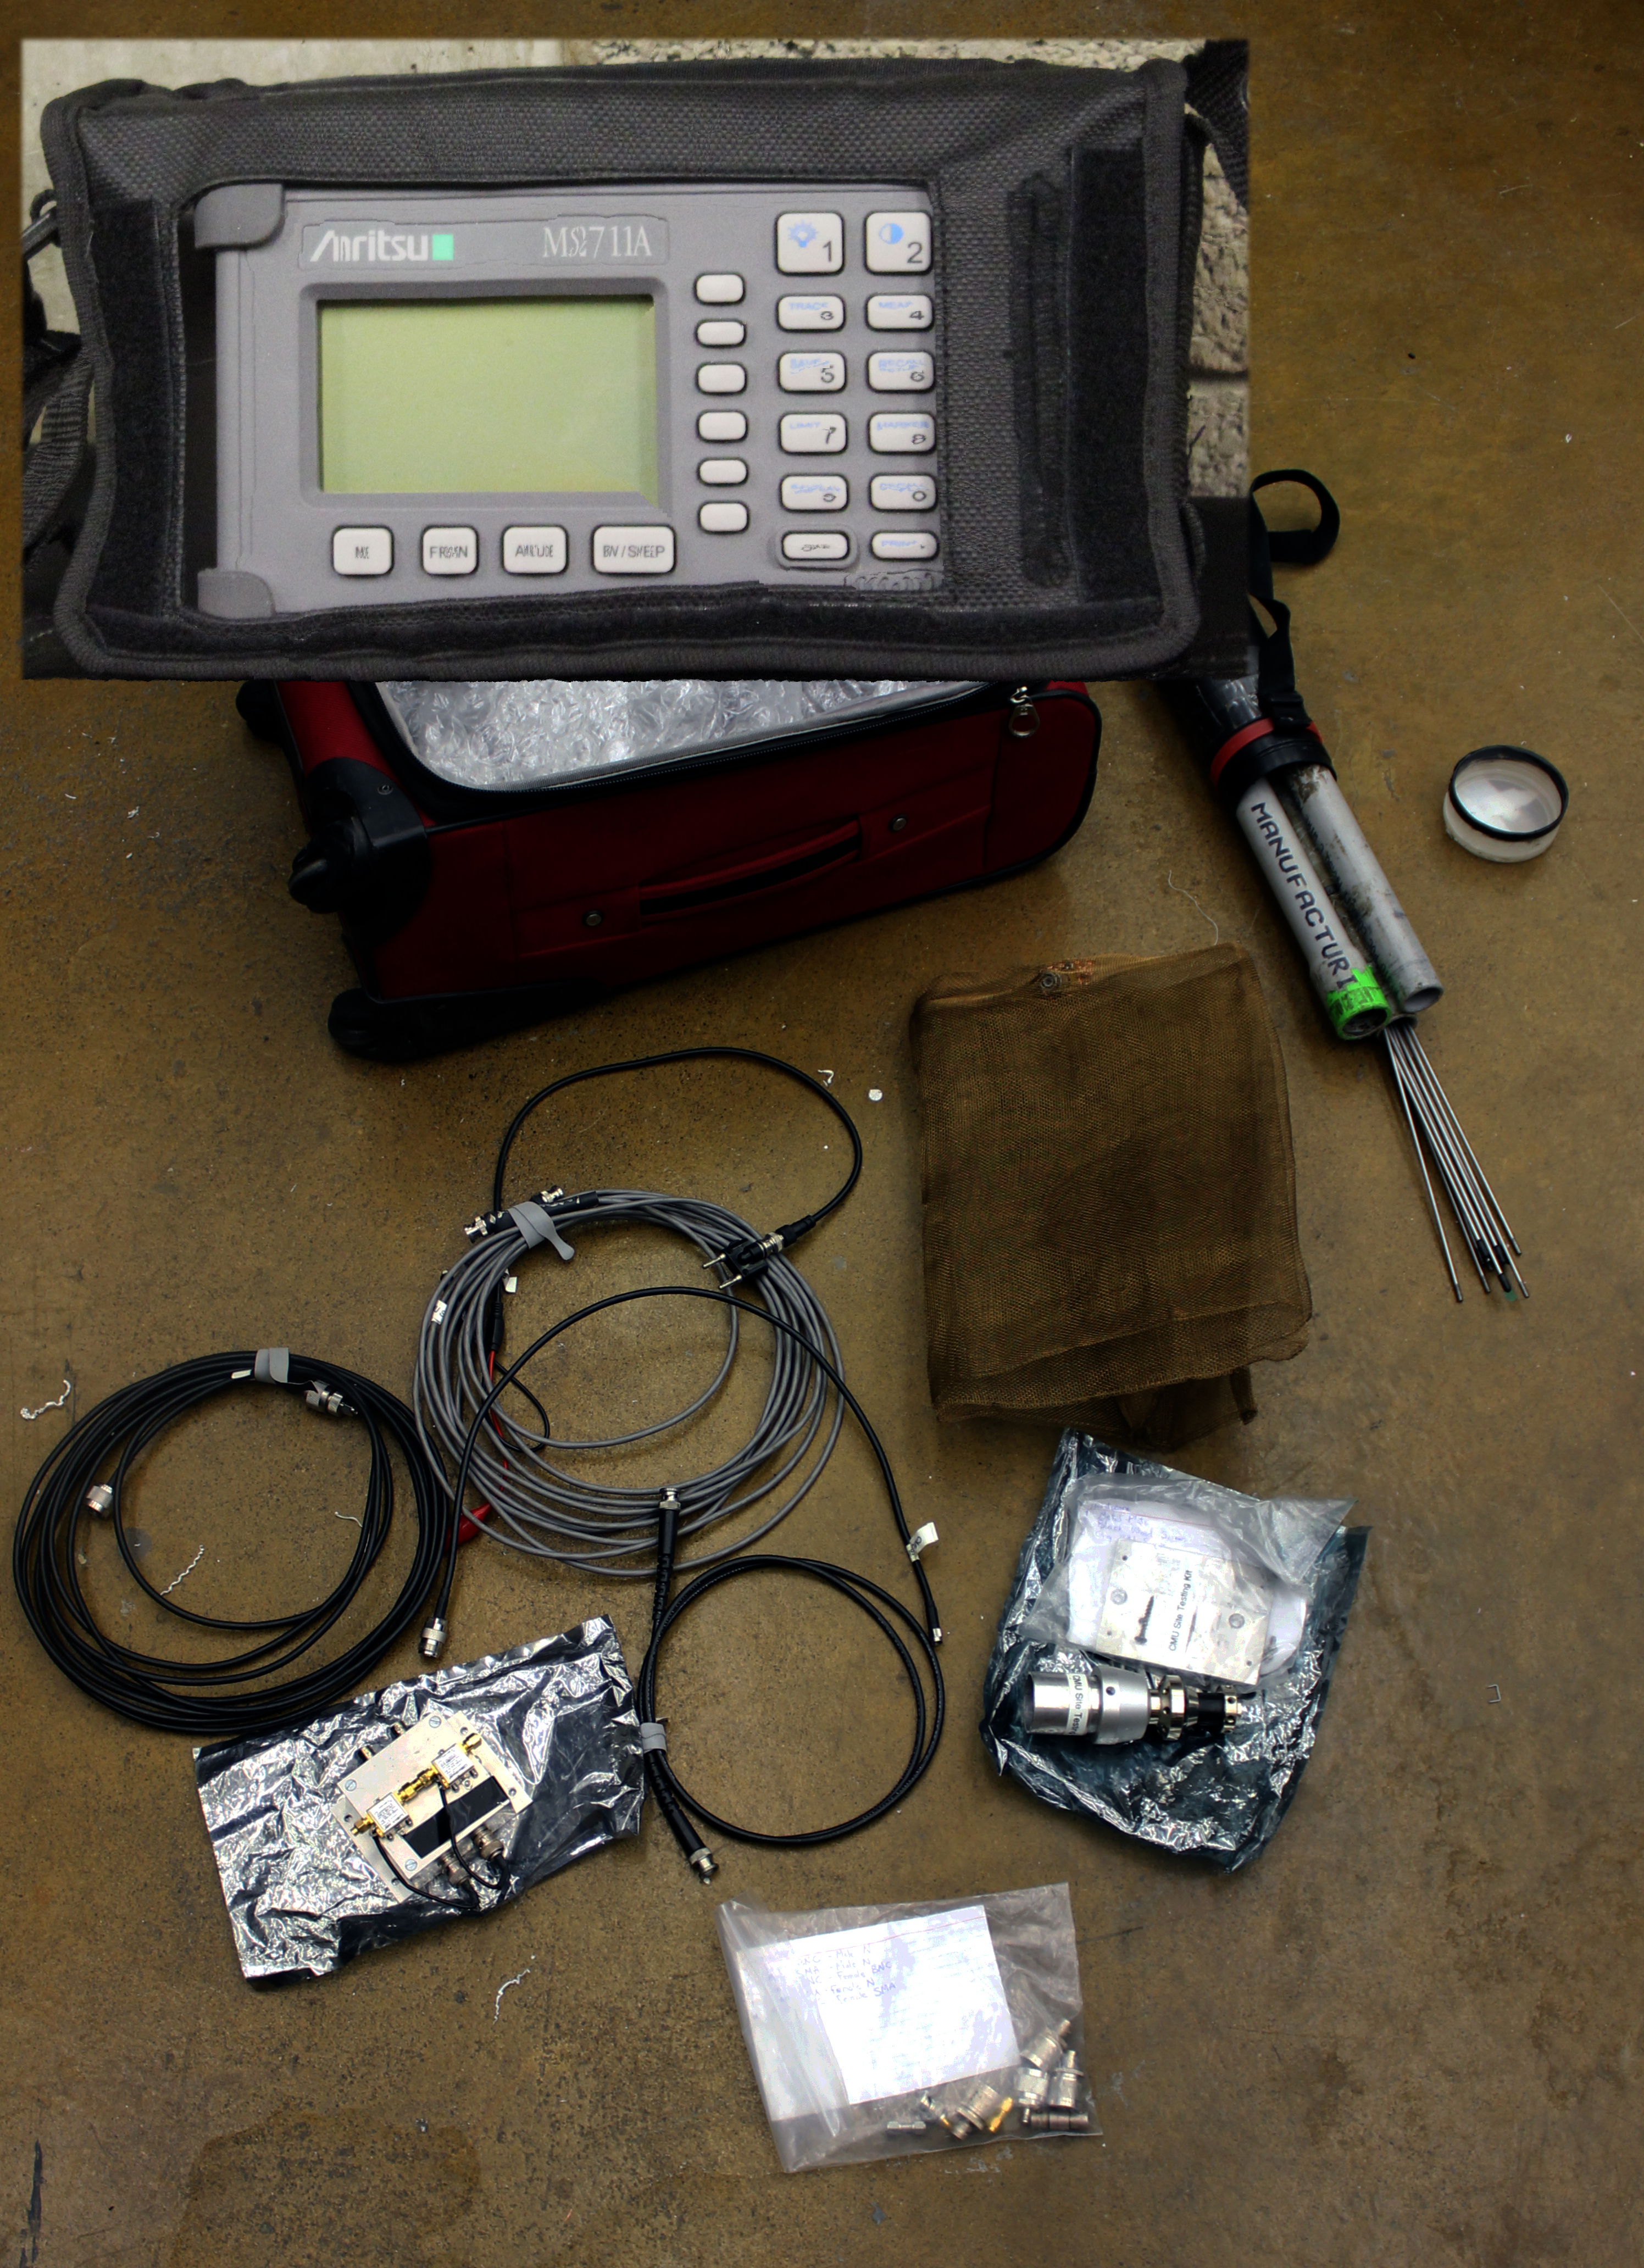
\includegraphics[width=0.95\linewidth]{RFI_testing/figures/site_testing_kit.jpg}
\caption{Site testing kit (except for the portable Spectrum Analyzer) laid out in the lab.}
\label{Fig:site_kit}
\end{minipage}%
\begin{minipage}[b]{0.02\textwidth}
\hspace{1cm}
\end{minipage}%
\begin{minipage}[b]{0.47\textwidth}
\centering
\includegraphics[width=0.95\linewidth]{RFI_testing/figures/voytek_site_test_alg.jpg}
\caption{Collecting data with the site testing equipment at the ARO site.}
\label{Fig:aroant}
\end{minipage}
\end{figure}

\begin{figure}[htb]
\begin{center}
\includegraphics[width=0.9\linewidth]{RFI_testing/figures/50Ohm_cal.png}
\caption{50 Ohm resistor as measured with site testing kit. FM spikes are RF leakage due to the measurement being made in the lab in Pittsburgh.}
\label{Fig:resflux}
\end{center}
\end{figure}

One major element of site evaluations was a short time-scale measurement of the RFI over a wide frequency band at each site. In order to do this, a sit testing kit was assembled. The kit includes a broadband antenna, amplifiers, and a portable spectrum analyzer for data collection. 

RFI signals are picked up by the antenna, a Workman $T-601$ discone antenna with a vertical polarization and a 3 meter plastic mast (see Figure \ref{Fig:aroant}). From the antenna, the signal is sent through a 1 meter cable to a set of amplifiers (Minicircuits $ZX60-33LN$ and $ZX60-4016E$) powered by a DC battery pack. The signal is then sent down a $\sim$7 meter cable to the spectrum analyzer. The spectrum analyzer (Anritsu $MS2711$) was enclosed in a brass mesh bag (Faraday Cage) to minimize self-generated RFI contamination. 

Data was collected in 200 MHz bands from $\sim$1 MHz to 1600 MHz, with a collection resolution of 10 kHz (although data is stored at a much lower resolution due to the limitations of the spectrum analyzer) and recorded in dBm. In order to convert the data to flux density (S in $dBW/m^2Hz$), Equation \ref{eq:fluxdens} was applied to the data. In the equation, $G$ is the amplifier gain in dB, $BW$ is the effective spectrum analyzer bandwidth in Hz and $G_{ant}$ is the antenna gain in dB. 

\begin{equation}\label{eq:fluxdens}
S \Bigg( \frac{dBW}{m^2 Hz} \Bigg) = P_{meas} (dBm) - 30 \Bigg( \frac{dBW}{dBm} \Bigg) - G - 10log_{10} [BW] - G_{ant}
\end{equation}

Amplifier gain ($G$) was measured in the lab using a noise figure meter and antenna gain ($G_{ant}$) can be calulated using Equation \ref{eq:gant}, where $\nu$ is the frequency in Hz, and $A_g$ is the isotropic antenna gain in $m^2$. We used the typical discone antenna value here, which is $1 dBi$ or $10^(1dBi/10) m^2$. 

\begin{equation}\label{eq:gant}
G_{ant}= 10 log_{10} \Bigg[ \Bigg(\frac{c}{\nu} \Bigg)^2 \Bigg( \frac{A_g}{4 \pi} \Bigg) \Bigg]
\end{equation}

To test the conversion equation, we replaced the antenna with a $50 \Omega$ resistor. That resistor should see a flux density as shown in Equation \ref{eq:resflux}, where k is the Boltzmann Constant T is the room temperature in Kelvin and NF is the amplifier noise as measured by the noise figure meter. 

\begin{equation}\label{eq:resflux}
S \Bigg( \frac{dBW}{m^2 Hz} \Bigg) = 10 log_{10} [k T] + NF 
\end{equation}

\begin{figure}[tb]
\begin{center}
\includegraphics[width=0.95\textwidth]{RFI_testing/figures/large_scale_site_map.jpg}
\caption{Map of evaluated sites in North America.}
\label{Fig:site_map}
\end{center}
\end{figure}

The results of this measurement are shown in Figure \ref{Fig:resflux}. The measured signal was slightly higher than expected signal. Some of this difference was tied to the effective spectrum analyzer bandwidth (30 kHz rather than the expected 10 kHz). The remainder of the difference may come from additional noise in the system or uncertainty in the noise figure meter values and appears to be roughly flat in frequency. 


Because we use the same kit at all the sites, any systematic noise contribution such as the uncertainty in the 50 Ohm data found in Figure \ref{Fig:resflux} is constant across all datasets and can be ignored in our data. 

\section{Existing Site Evaluations}

\begin{figure}[tb]
\begin{center}
\includegraphics[width=0.9\linewidth]{RFI_testing/figures/Pittsburgh_cal.png}
\caption{RFI measurement at Carnegie Mellon University in Pittsburgh, Pennsylvania}
\label{Fig:pghcal}
\end{center}
\end{figure}


Using the site testing kit discussed in the previous section, data was taken at each of the sites shown in Figure \ref{Fig:site_map}. The portability of the kit (it packs up into the small suitcase and poster tube shown in Figure \ref{Fig:site_kit}) allows it to be easily transported to each of the sites. 

\subsection{Carnegie Mellon University Pittsburgh, PA, USA}

Carnegie Mellon University is located in the city of Pittsburgh ($40^\circ 26'30''$ N, $80^\circ 00' 00''$ W), home to several such universities and possessing a population of over 300,000. As should be expected, the radio environment in Pittsburgh is full of RFI with signals of such magnitude that they overload test equipment. Figure \ref{Fig:pghcal} shows the RFI environment in Pittsburgh as measured with the site testing kit. In order to not overload the spectrum analyzer with the high RFI levels at some frequencies, it was necessary to remove one stage of amplification from the system. 


\begin{figure}[htb]
\centering
\begin{minipage}[b]{0.47\textwidth}
\centering
\includegraphics[width=0.75\linewidth]{RFI_testing/figures/National_Radio_Quiet_Zone.png}
\caption{Extent of the US National Radio Quiet Zone around the Green Bank Site.}
\label{Fig:nrqz}
\end{minipage}%
\begin{minipage}[b]{0.02\textwidth}
\hspace{1cm}
\end{minipage}%
\begin{minipage}[b]{0.47\textwidth}
\centering
\includegraphics[width=0.95\linewidth]{RFI_testing/figures/gbt_site.jpg}
\caption{Robert C. Byrd Green Bank Radio Telescope. }
\label{Fig:gbt}
\end{minipage}
\end{figure}

\begin{figure}[htb]
\begin{center}
\includegraphics[width=0.9\linewidth]{RFI_testing/figures/GBT_cal.png}
\caption{RFI measurement at the NRAO Green Bank site. }
\label{Fig:gbtrfi}
\end{center}
\end{figure}

\subsection{National Radio Astronomy Observatory (NRAO) Green Bank, WV, USA}

The National Radio Astronomy Observatory (NRAO) is a research center funded by the United States National Science Foundation (NSF). It maintains several telesopes in radio quiet locations. One of these locations is in Green Bank, West Virginia inside the United States National Radio Quiet Zone in Virginia and West Virginia (see Figure \ref{Fig:nrqz}). Within this zone radio broadcasts at all frequencies are extremely limited, allowing for a relatively quiet RFI environment. 

The Green Bank site ($38^\circ 25' 59''$ N, $79^\circ 50' 23''$ W) hosts a number of radio telescopes including the 100 m Robert C. Byrd Green Bank Radio Telescope (see Figure \ref{Fig:gbt}). As an NRAO facility, the site has a full staff and facilities including housing, power, and other amenities. Located off a local highway, the site is a simple 4-5 hour drive from Pittsburgh. 

Looking at the data from the site testing kit, we found that the size of the radio quiet zone (about 34,000 $km^2$) is sufficient for higher frequencies but becomes to small at lower frequencies. As you can see in Figure \ref{Fig:gbtrfi}, there are specific bands of frequencies below 600 MHz where there is a great deal of RFI. One of these highly contaminated bands is the FM radio band. 

\begin{figure}[htb]
\begin{center}
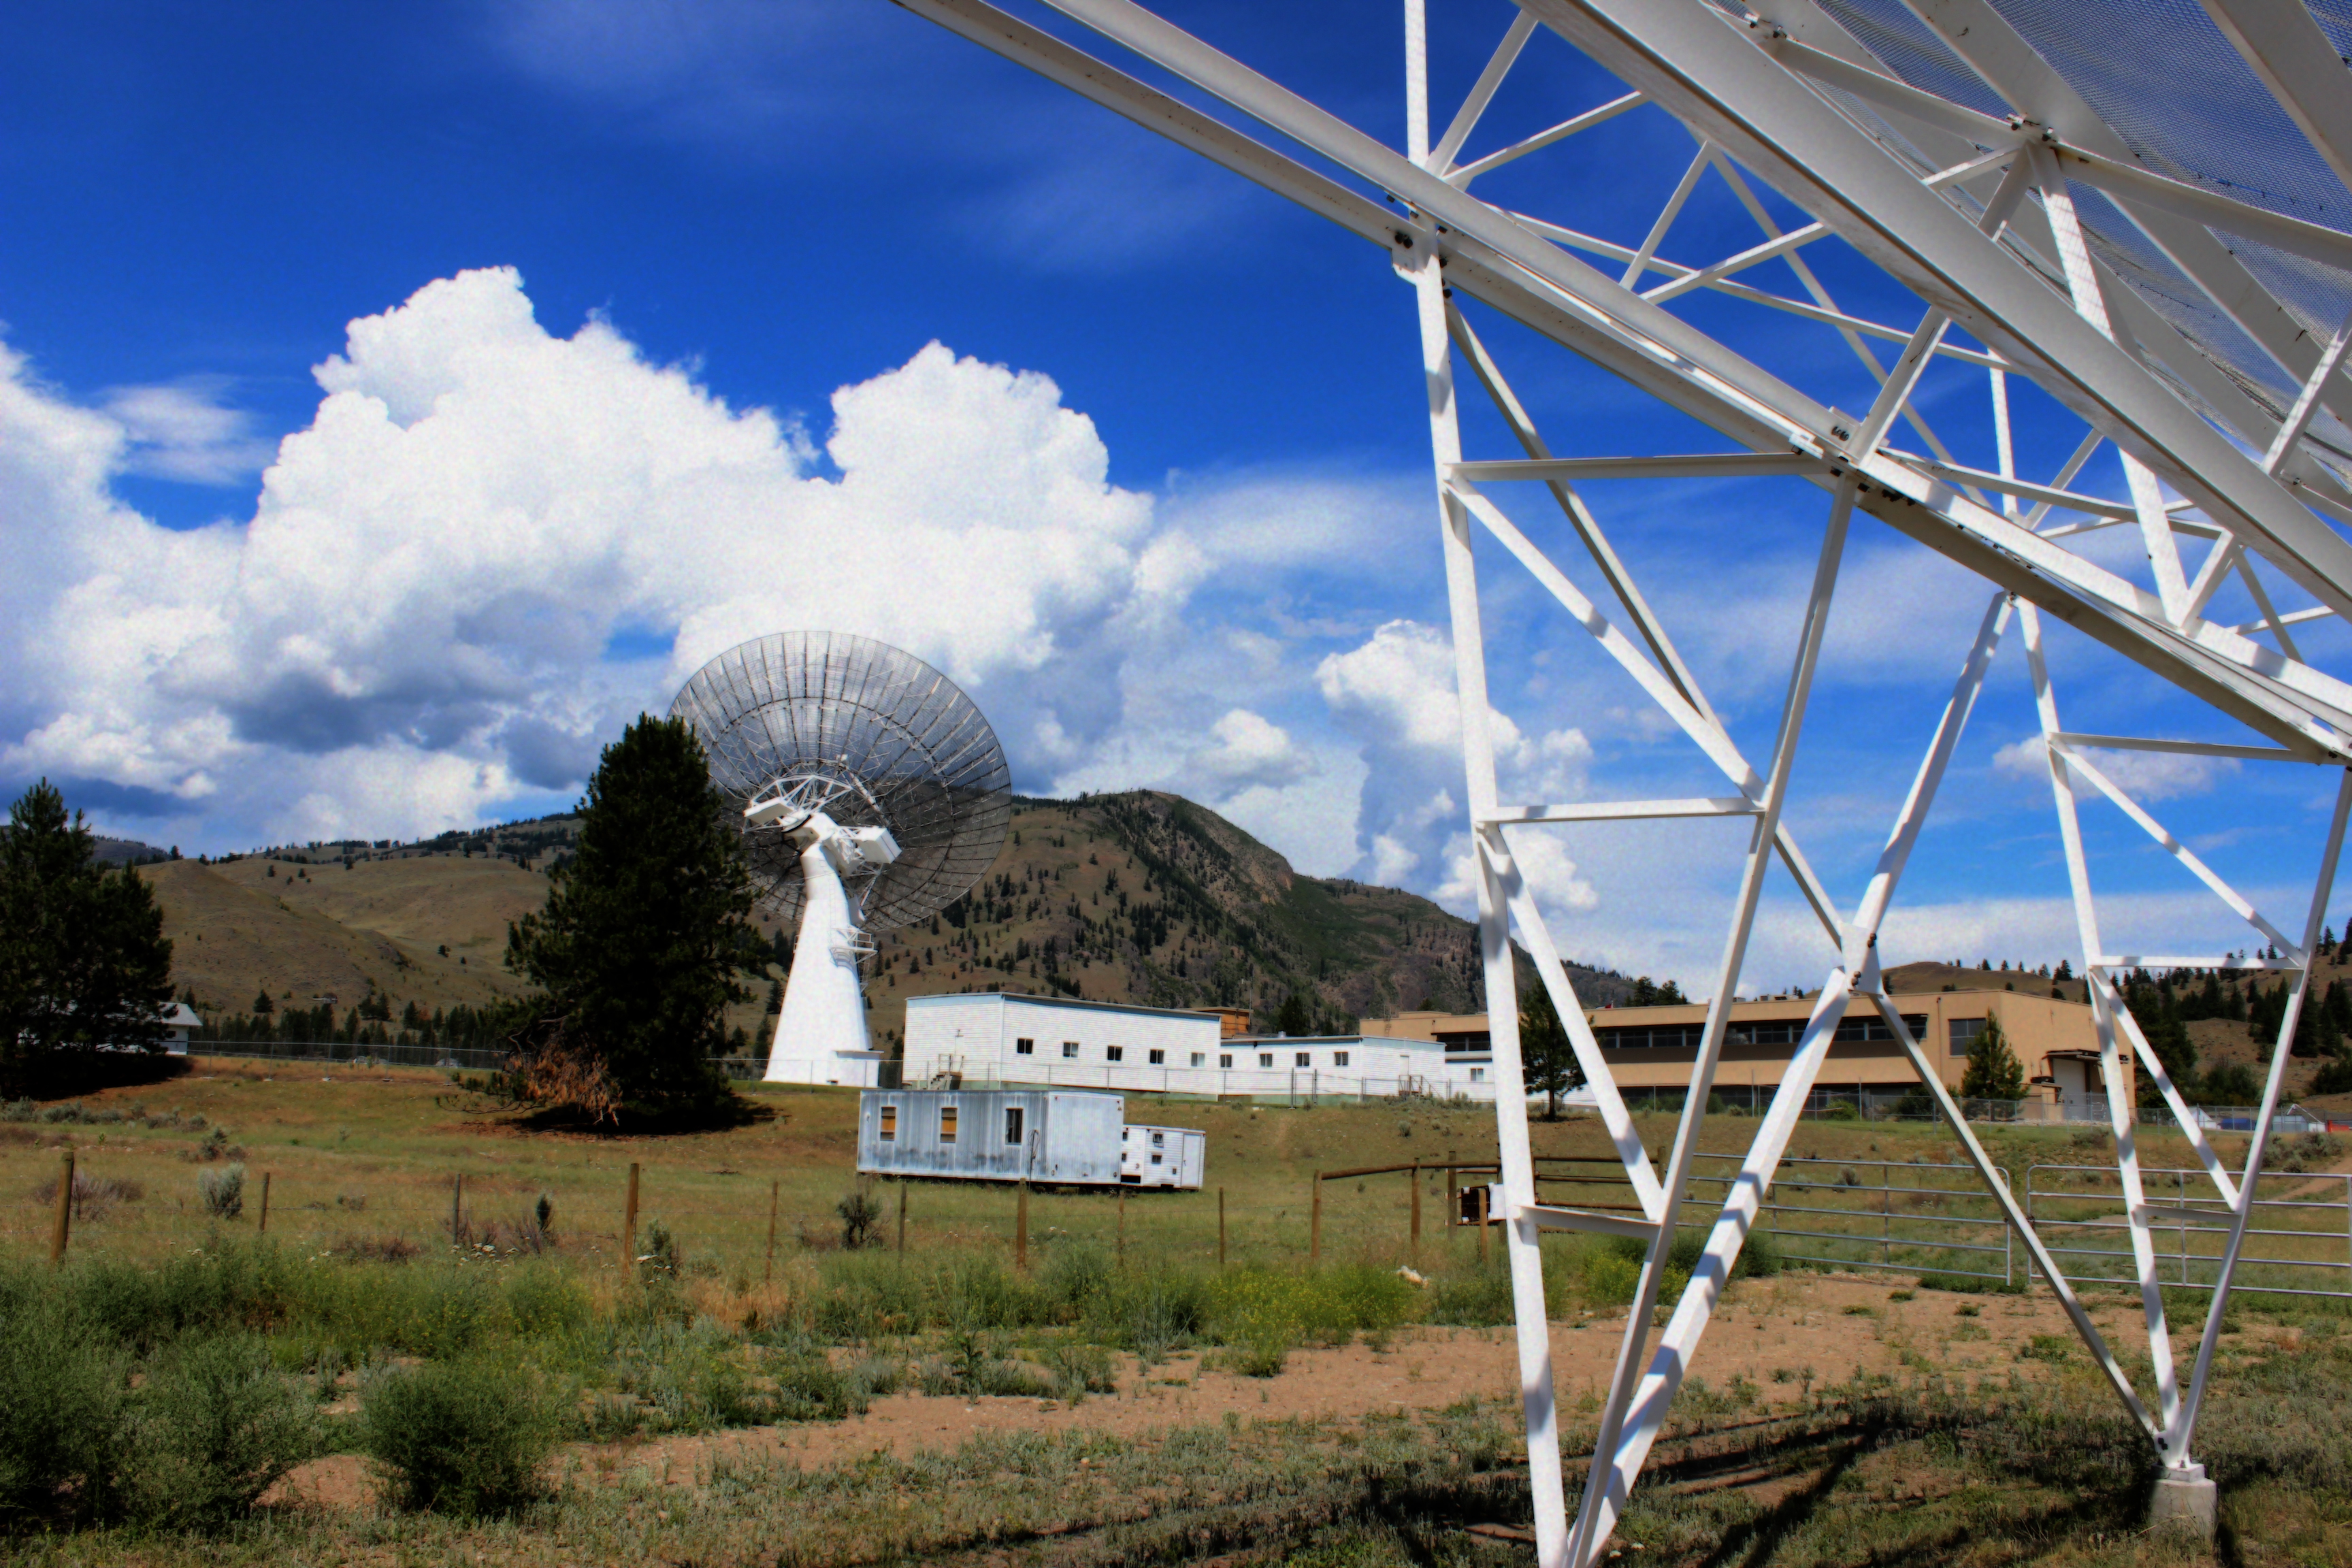
\includegraphics[width=0.9\linewidth]{RFI_testing/figures/penticton_rect.jpg}
\caption{Some of the DRAO facilities and telescopes (CHIME pathfinder in foreground). }
\label{Fig:penticton}
\end{center}
\end{figure}

\begin{figure}[htb]
\begin{center}
\includegraphics[width=0.9\linewidth]{RFI_testing/figures/DRAO_cal.png}
\caption{RFI measurement at the DRAO Penticton site. }
\label{Fig:draorfi}
\end{center}
\end{figure}

\begin{figure}[tb]
\begin{center}
\includegraphics[width=0.9\linewidth]{RFI_testing/figures/ALG_cal.png}
\caption{RFI measurement at the ARO Algonquin site.}
\label{Fig:arorfi}
%\end{minipage}
\end{center}
\end{figure}

\subsection{Dominion Radio Astrophysical Observatory (DRAO)}

The Dominion Radio Astrophysical Observatory (DRAO) is a Canadian radio astronomy site ($49^\circ 19' 15.6''$ N, $119^\circ 37' 26.4''$ W). Located near Penticton, British Columbia in the south-central part of the province, DRAO has a number of radio telescopes on site and the Canadian Hydrogen Intensity Mapping Experiment (CHIME) system is currently being built there. Figure \ref{Fig:penticton} shows some of the facilities at DRAO including part of the CHIME pathfinder in the foreground. 

The site can be easily accessed by car, with on-site facilities available for researchers. It is also a $\sim$30 minute drive from Penticton, a town with a population of over 30,000. 

Like the NRAO Green Bank site, the DRAO site has insufficient isolation from civilization to provide a radio quiet environment at the lower frequencies. There is significant RFI contamination for most frequencies below 500 MHz at this site (see Figure \ref{Fig:draorfi}).  

\subsection{Algonquin Radio Observatory (ARO)}

The Algonquin Radio Observatory (ARO) is a single instrument Canadian radio astronomy site ($45^\circ 57' 19.8''$ N, $78^\circ 4' 23''$ W). Located in the center of Algonquin Provincial Park in Ontario, Canada; the site is only accessible by logging roads, which are gravel but can be driven by most vehicles during the summer. ARO does have power and full amenities on site including housing for researchers. 

Although the site has excellent radio quiet properties at higher frequencies, it is still relatively close (about 200-250 km) to the major Canadian metropolitan areas of Toronto and Ottawa. When we set up our site test at ARO (see Figure \ref{Fig:arorfi}, we found that although the rest of the spectrum is quite clean there is still significant RFI below 300 MHz (see Figure \ref{Fig:arorfi}), including in the FM radio band. 


\begin{figure}[htb]
\begin{center}
\includegraphics[width=0.9\linewidth]{RFI_testing/figures/zds_overview_shot.jpg}
\caption{View of the Zona del Silencio from one of the nearby peaks. The ecologist's camp where we stayed while running our tests is in the center of the picture.}
\label{Fig:zdsover}
\end{center}
\end{figure}

\begin{figure}[htb]
\begin{center}
\includegraphics[width=0.9\linewidth]{RFI_testing/figures/ZdS_halfway_in_cal.png}
\caption{RFI measurement near the ecologist's camp in the Zona del Silencio.}
\label{Fig:zdsendrfi}
\end{center}
\end{figure}

\section{New Site Evaluations}

Evaluation of these existing radio quiet sites demonstrated a clear need for sites whose RFI environments are clean to lower frequencies. However, locating such sites can be difficult as the distances required begin to grow large. I will report on a couple of potential sites in Mexico that have significant improvement in their low frequency RFI strength compared to the existing sites. 

\subsection{La Zona de Silencio Mapimi, Mexico}
$''$Zona del Silencio$''$ ($26^\circ 41' 10.3''$ N, $103^\circ 44' 50.9''$ W) is a radio quiet region in the Mapimi part of the Chihuahuan desert in Northern Mexico. Its current radio quiet status is a feature of geography as it is surrounded by mountains and has no major metropolitan areas in the local region. It is also a protected biosphere reserve maintaned by Mexcio's $''$Comisi\'{o}n Nacional de \'{A}reas Naturales Protegidas$''$ (CONANP). 

\subsubsection{Logistics and Current Infrastructure}
While major highways can be found along the outside of the region, the only roads in and out of the site are poorly maintained dirt roads that require 4-wheel drive at a minimum. 

Permanent settlements are not allowed within the biosphere reserve. However, at the center of the site is a camp for ecologists studying the biosphere found in the reserve. The site has minimal housing with solar cells charging batteries for power but all water on site has to be brought in from outside. 

For our site test, we got special permission to stay at the ecologist's camp called $''$Laboratorio del Desierto$''$, shown in Figure \ref{Fig:zdsover}.

\subsubsection{Environmental Impacts}

During the site testing, we were able to observe the general climate of the site as a consideration for future deployments. One of the challenges we observed was the prevalence of dust due to the arid climate. All our equipment had to be well protected from dust, especially during transport to and from the site. If not properly shielded, dust can cause electronic equipment to malfunction. 

Another potential challenge is the temperature variation associated with the climate. Even within a single day we saw a strong difference between night and and day temperatures. Temperature variation can create variance in collected data from a telescope, making the desired signals more difficult to detect. 

\subsubsection{Measurements}

On this first site test, we chose to measure the site quality at a specific location near the center of the zone where RFI was expected to be at a miniumum. Setting up near the ecology camp but far enough away to prevent contamination by the local electronics, we measured extremely low RFI levels as is shown in Figure \ref{Fig:zdsendrfi}.

There is still some noise at lower frequencies, but the FM band is considerably quieter than at any of the existing radio quiet sites that we had tested. 

Further testing at this site should include a survey of a wide range of locations within the $''$Zona del Silencio$''$ to map out the region's radio quiet properties. 

\begin{figure}[htb]
\centering
\begin{minipage}[b]{0.47\textwidth}
\centering
\includegraphics[width=0.95\linewidth]{RFI_testing/figures/isla_guadalupe_site_map.jpg}
\caption{Map of Isla Guadalupe with the relevant sites indicated.}
\label{Fig:guadmap}
\end{minipage}%
\begin{minipage}[b]{0.02\textwidth}
\hspace{1cm}
\end{minipage}%
\begin{minipage}[b]{0.47\textwidth}
\centering
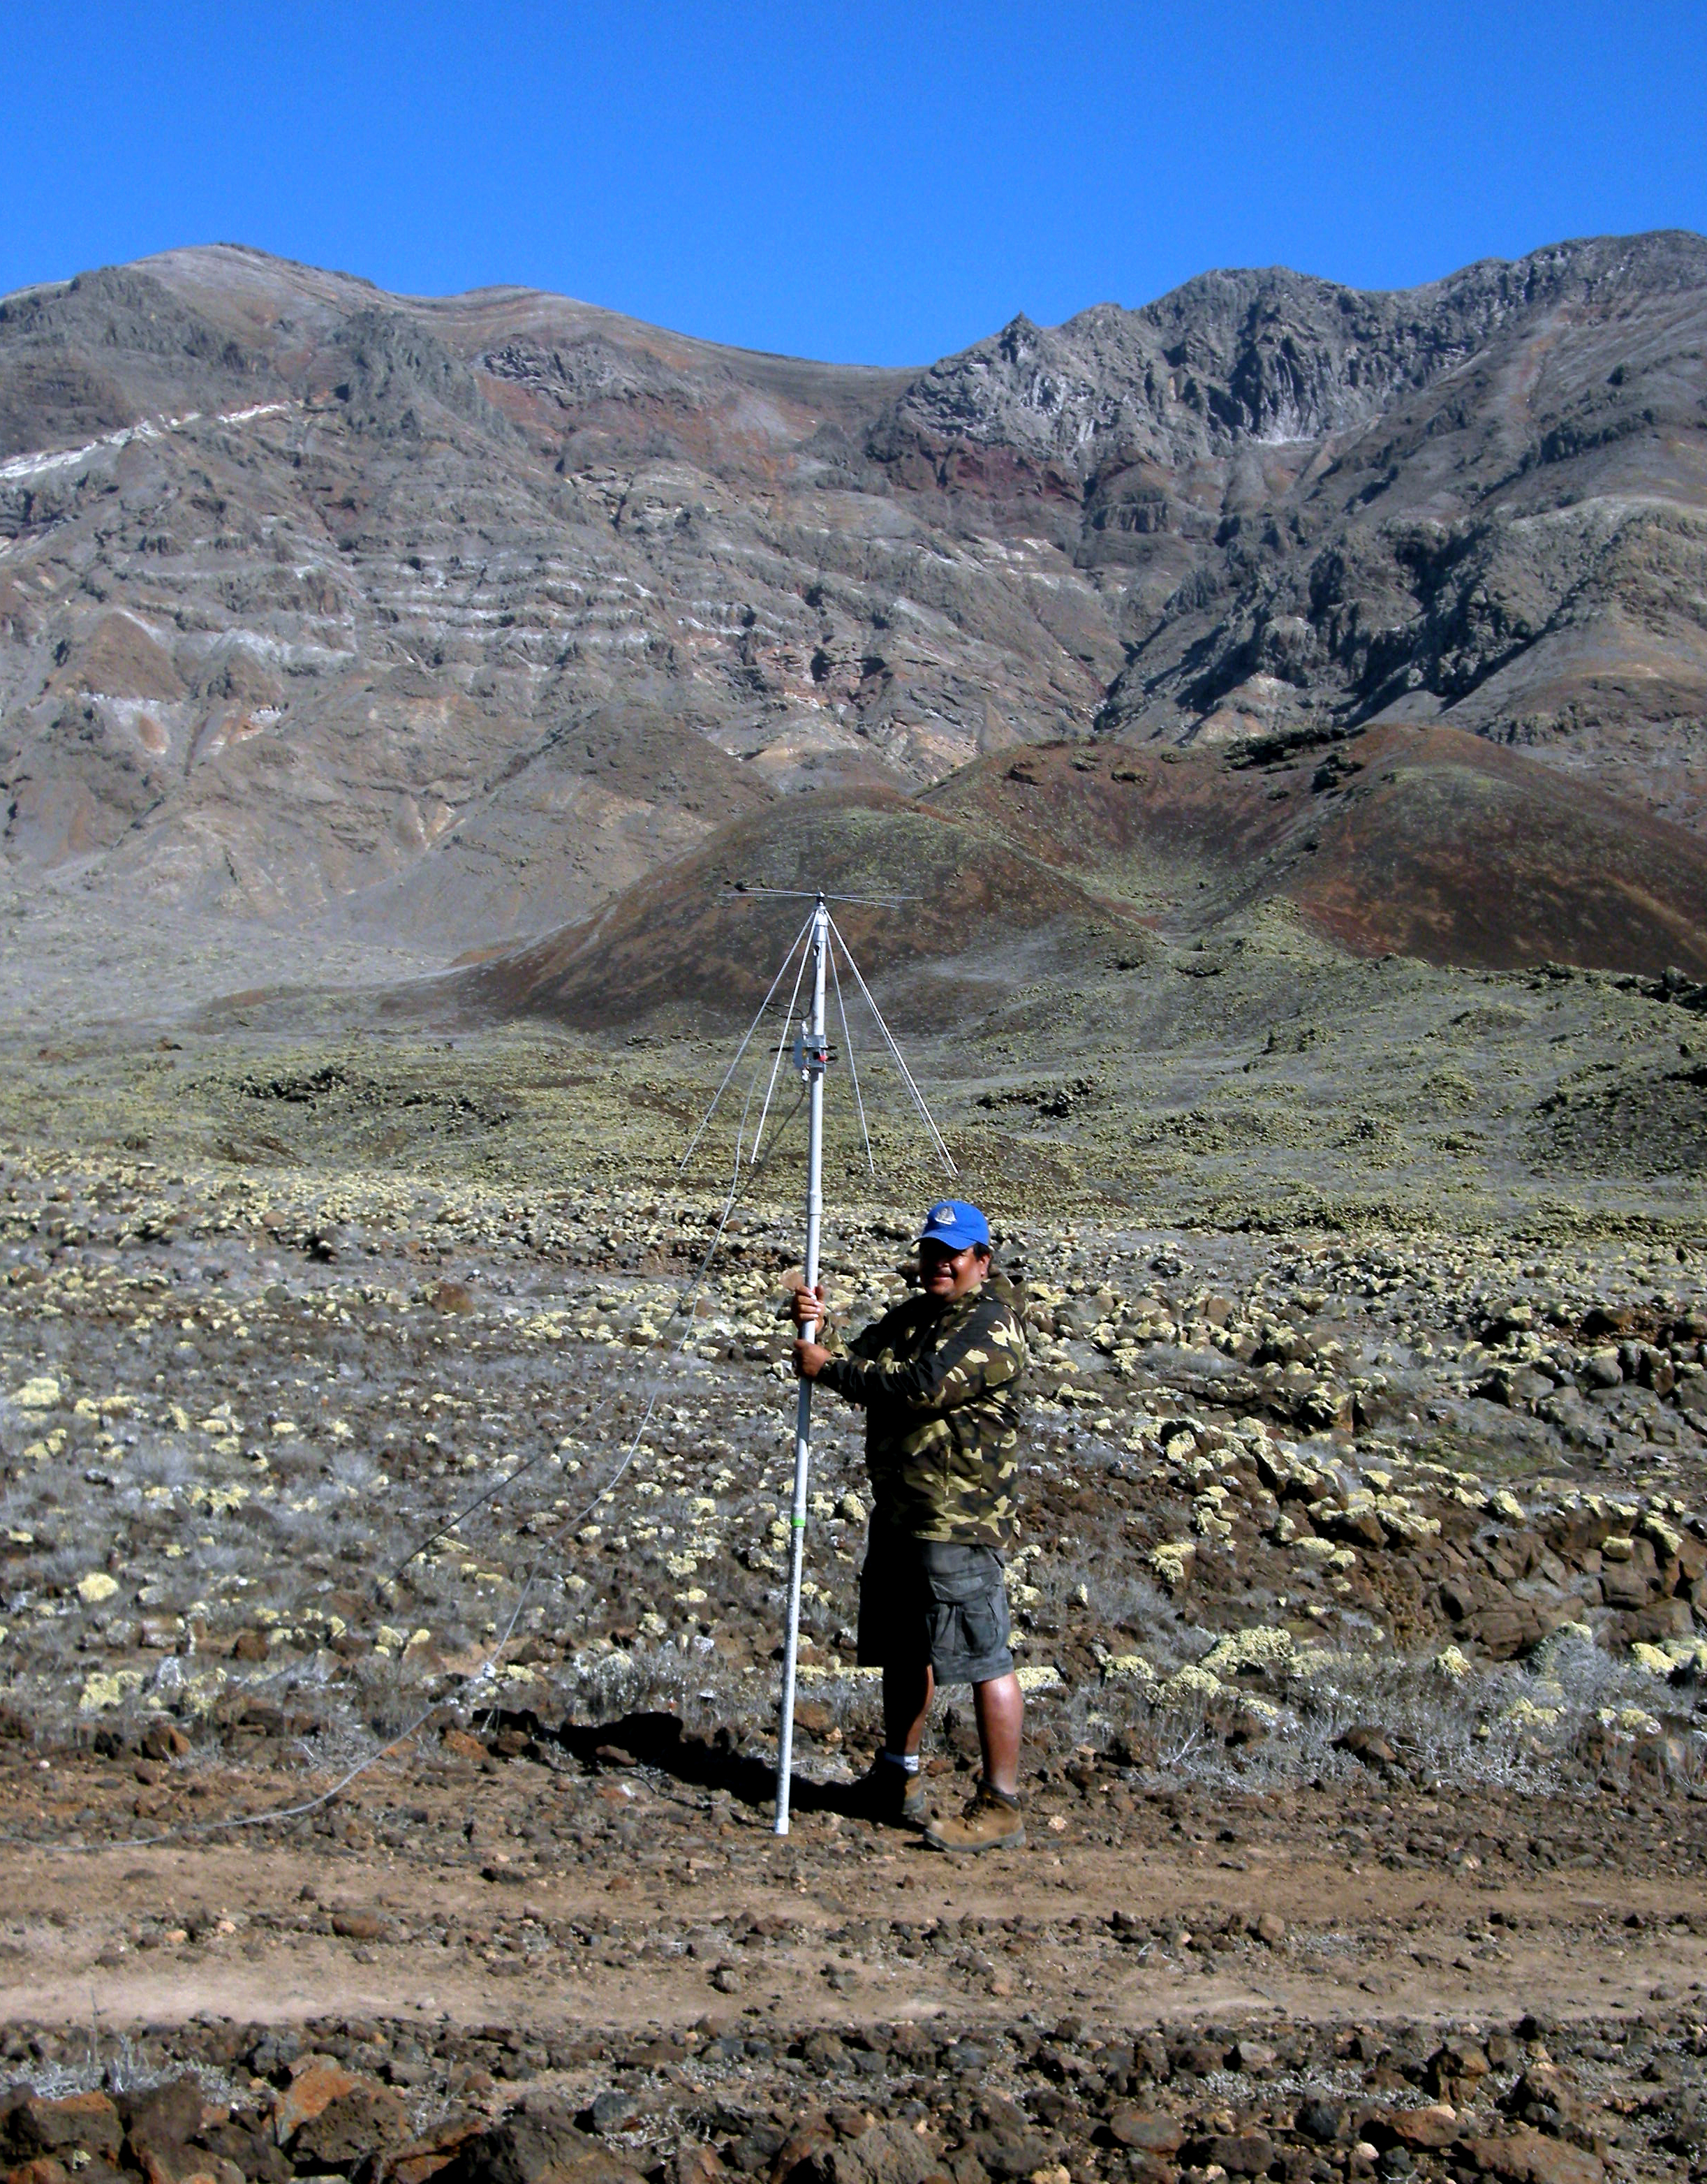
\includegraphics[width=0.95\linewidth]{RFI_testing/figures/omar_site_test_guad.jpg}
\caption{Collecting data with the site testing equipment on Isla Guadalupe.}
\label{Fig:guadsite}
\end{minipage}
\end{figure}


\begin{figure}[tb]
\centering
\begin{minipage}[b]{0.47\textwidth}
\centering
\includegraphics[width=0.95\linewidth]{RFI_testing/figures/guad_plane.jpg}
\caption{Airplane used for access to Isla Guadalupe after landing on the island.}
\label{Fig:guadplane}
\end{minipage}%
\begin{minipage}[b]{0.02\textwidth}
\hspace{1cm}
\end{minipage}%
\begin{minipage}[b]{0.47\textwidth}
\centering
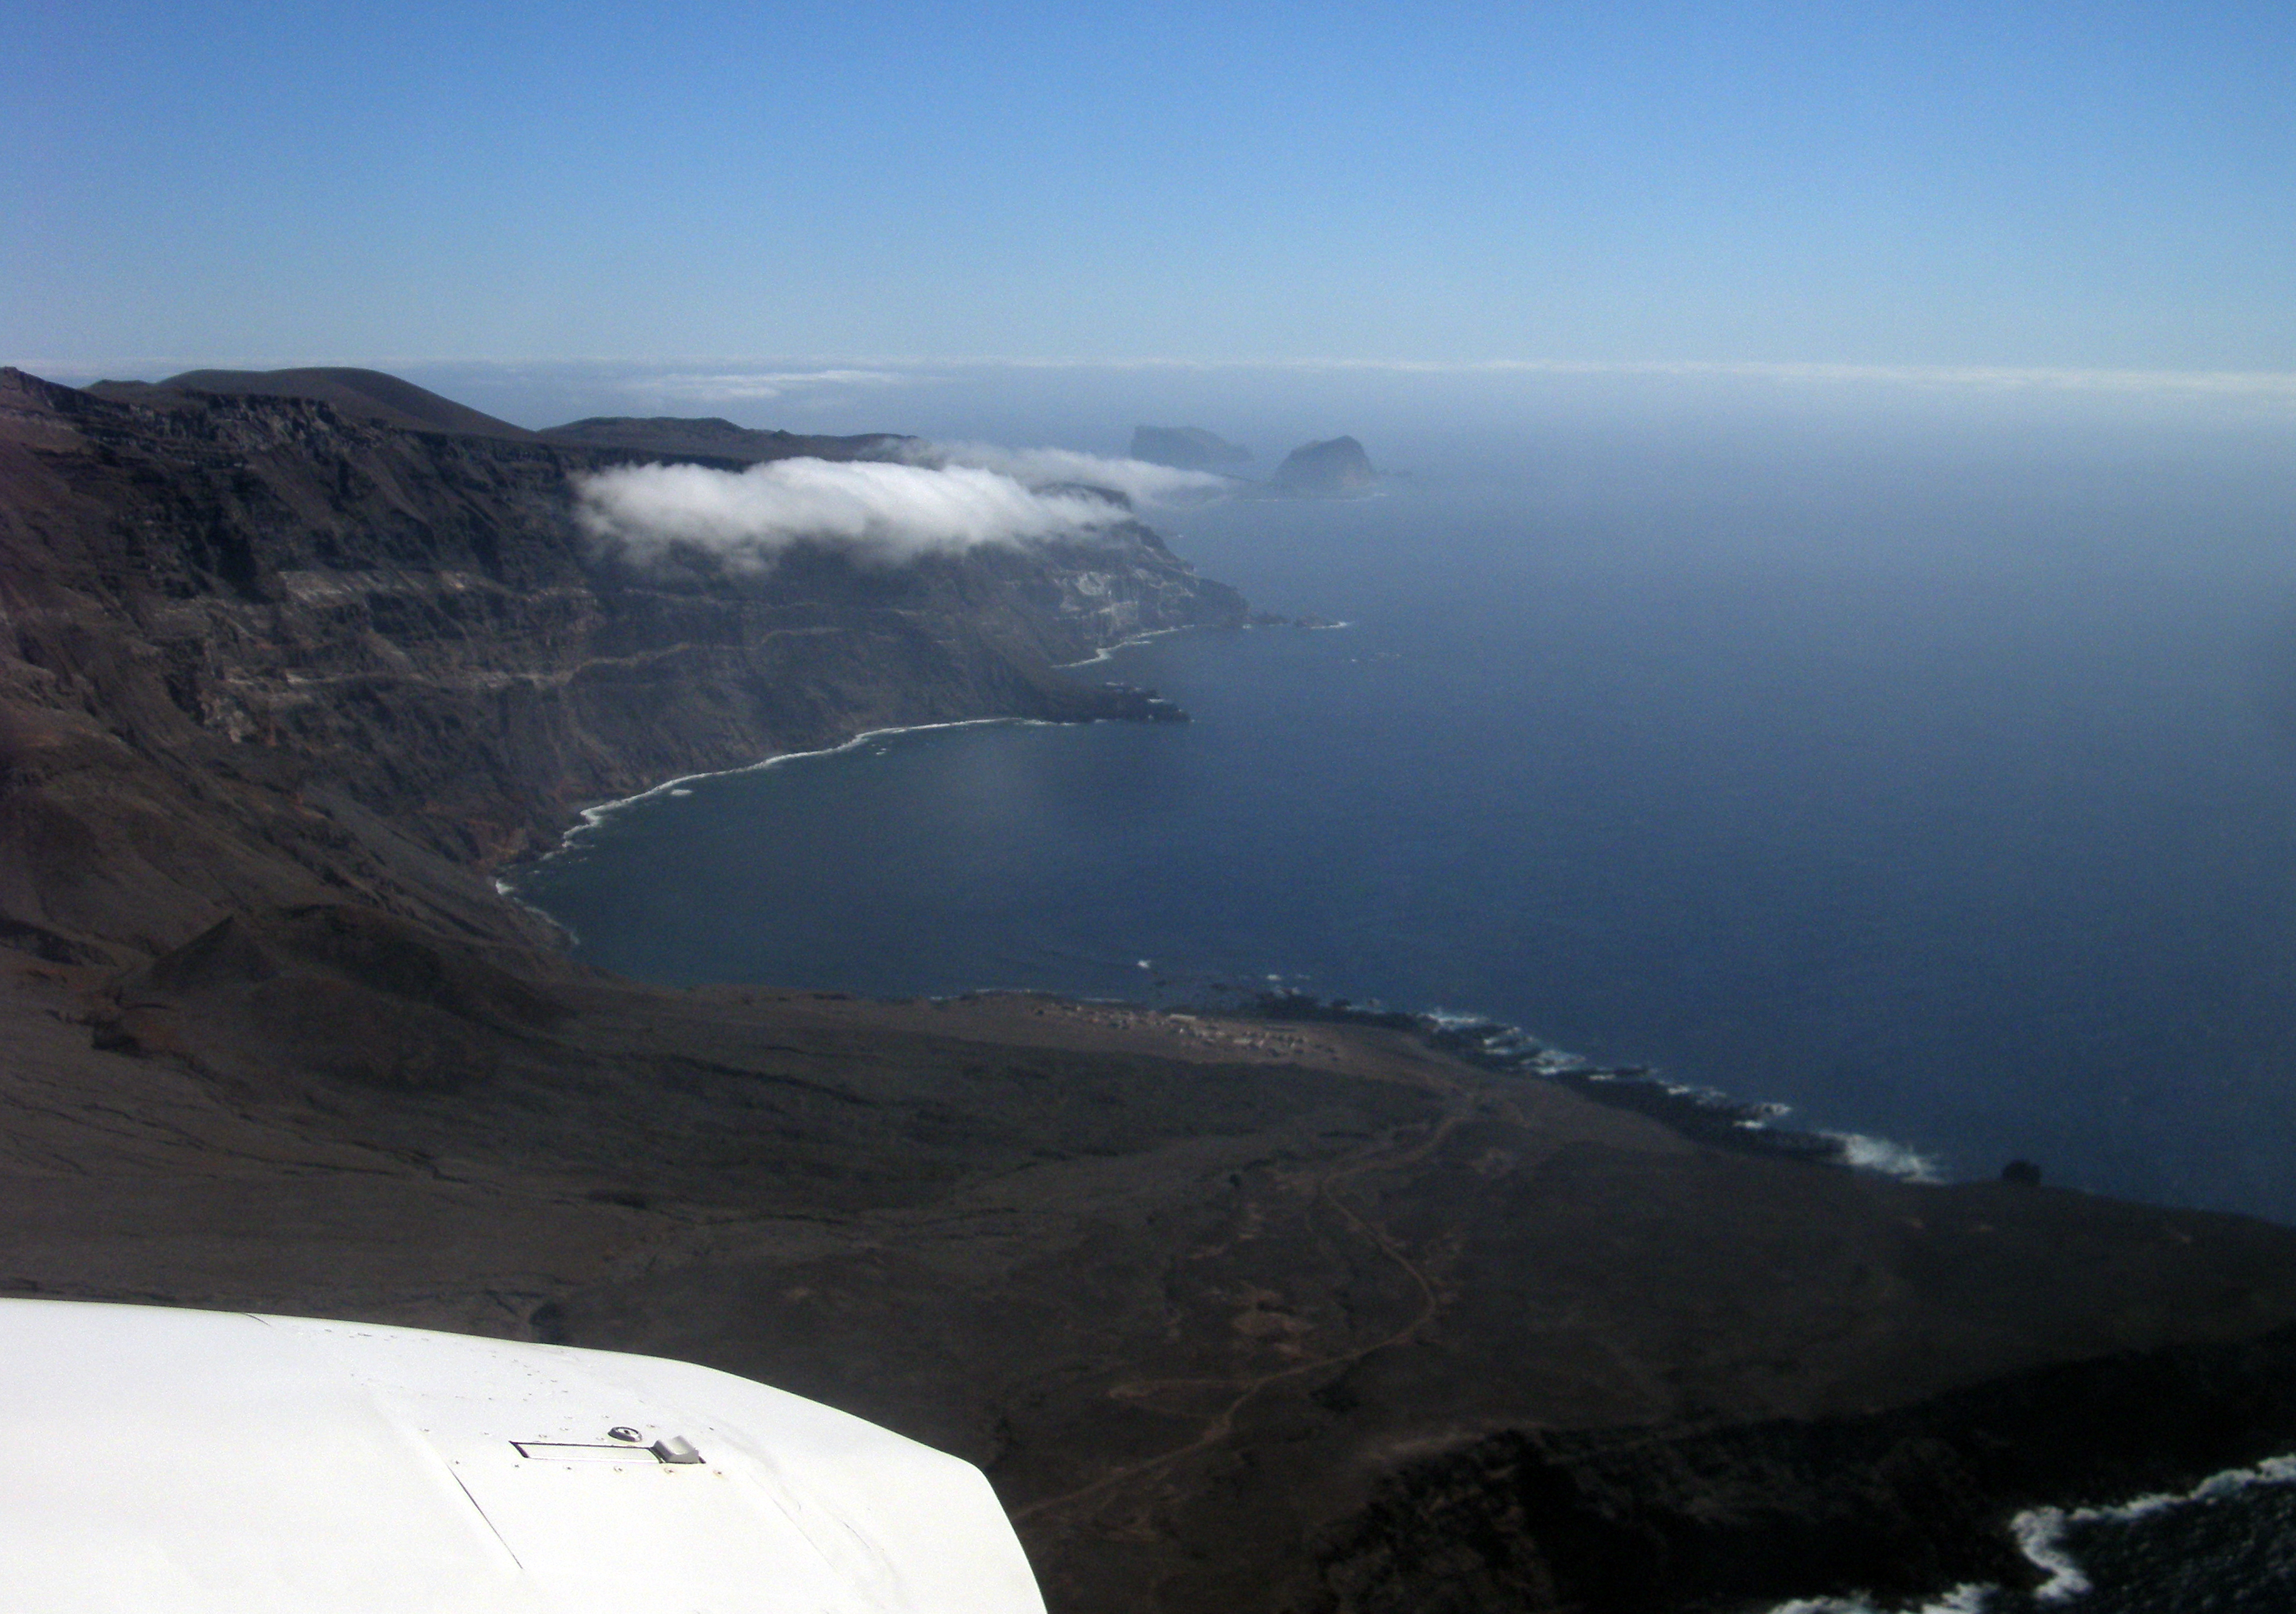
\includegraphics[width=0.95\linewidth]{RFI_testing/figures/guad_plateau_plane.jpg}
\caption{View of the plateau with the fishing village from the airplane.}
\label{Fig:guadplateau}
\end{minipage}
\end{figure}

\subsection{Isla Guadalupe Baja California, Mexico}

Isla Guadalupe ($29^\circ 1' 51''$ N, $118^\circ 16' 48''$ W) is a small volcanic island located about 250 $km$ west of Baja California in Mexico. The island is about 250 $km^2$, with two significant peaks along the north-south axis of the island. A biosphere reserve, access to Guadalupe is limited to a few groups; namely the Mexican government and Navy ($''$Secretar\'{i}a de Gobernaci\'{o}n$''$ and $''$Secretar\'{i}a de Marina$''$), ecologists studying the land and marine life such as the $''$Grupo de Ecolog\'{i}a y Conservaci\'{o}n de Islas A.C.$''$ (GECI) and CONANP, and the local fishing cooperative ($''$Sociedad Cooperativa d Producci\'{o}n Pesquera de Participaci\'{o}n Estatal Abuloneros y Langosteros, S.C.L.$''$). We were able to travel to Isla Guadalupe with support from these organizations. 

\begin{figure}[htb]
\centering
\begin{minipage}[b]{0.47\textwidth}
\centering
\includegraphics[width=0.95\linewidth]{RFI_testing/figures/mex_navy_arrival.jpg}
\caption{Mexican naval vessel as it arrived at Isla Guadalupe to deliver supplies.}
\label{Fig:guadboat}
\end{minipage}%
\begin{minipage}[b]{0.02\textwidth}
\hspace{1cm}
\end{minipage}%
\begin{minipage}[b]{0.47\textwidth}
\centering
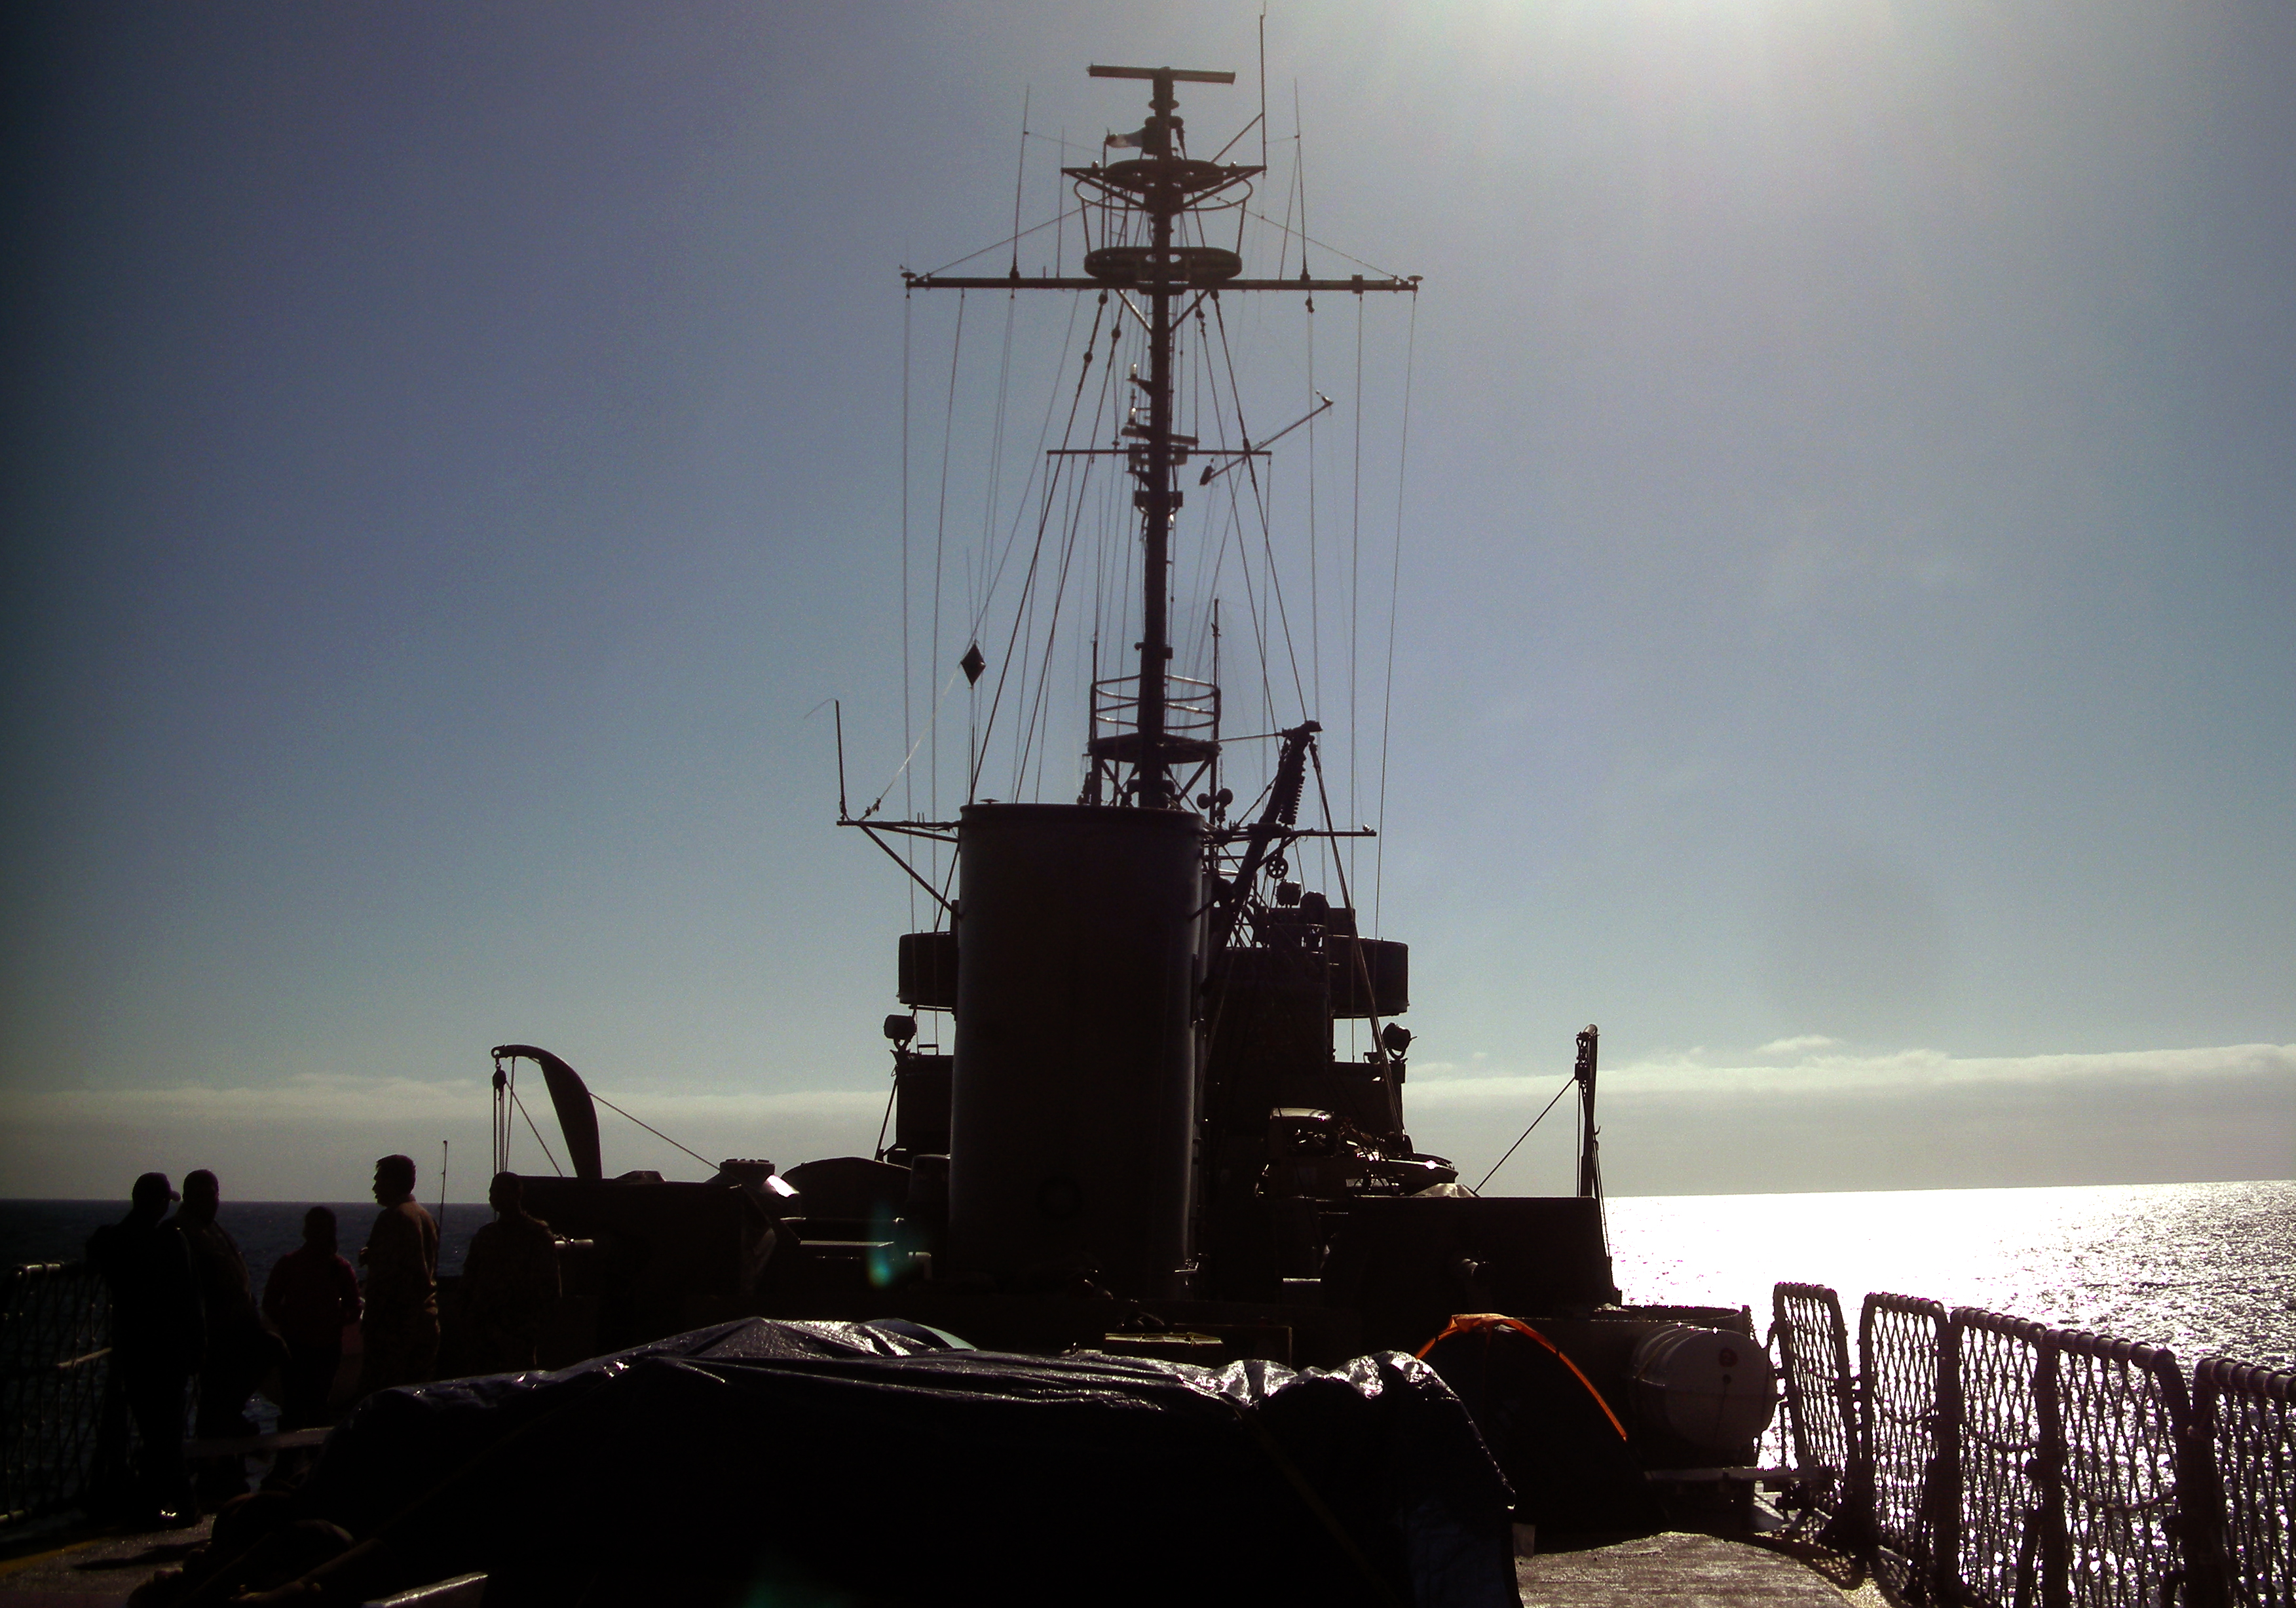
\includegraphics[width=0.95\linewidth]{RFI_testing/figures/mex_navy_onboard.jpg}
\caption{Onboard the Mexican naval vessel during trip back to the Port of Ensenada.}
\label{Fig:guadonboard}
\end{minipage}
\end{figure}

\subsubsection{Logistics and Current Infrastructure}

Access to Isla Guadalupe can requires one of two transport methods. First, small planes such as the one shown in Figure \ref{Fig:guadplane} can fly from the city of Ensenada in Baja California to the island, where there is a small landing strip. This flight takes 1-2 hours and can only be made during good weather. On several of our visits to Isla Guadalupe, this was our method of transport. 

A much cheaper alternative is transport with the supply ship that the Mexican Navy uses to support its base on Guadalupe. This supply ship, shown in Figures \ref{Fig:guadboat} and \ref{Fig:guadonboard}, deploys once a month from the port of Ensenada; stopping first at Isla Guadalupe, then Isla Cedros, then returning to Ensenada with a total travel time of about three days. Travel via this route requires passengers to $''$camp out$''$ by sleeping on the deck of the ship during transit. In addition, since passengers are hitching a ride with the ship they have no control over changes in ship deployment (eg delays or re-routing) that may change the departure or arrival schedule. This places strictures on any deployments to Isla Guadalupe that must be accounted for in planning the trip. 

While on Guadalupe we had the option of staying with the ecologists, the fishing village or the navy base. Each provided some level of logistical support, but all had limited resources. 

The ecology camp is a small camp with about 5-15 researchers in residence at any given time. Housing, including running water, is available at the site for the researchers and their visitors but there is little to no plumbing, so the bathroom is a dry toilet.  Since power is supplied by solar panels and batteries, it is pretty limited, especially at night. However, during the day there is regular internet access via satellite. Since it is a small camp, food is served communally, with everyone taking turns for cooking and cleaning responsibilities. 

In contrast, the fishing village has a semi-permanent population of about 100 people and can be seen in Figure \ref{Fig:guadplateau}. In the village there are a number of houses, one for each family currently on site on the island. Furnishings in the houses are haphazard since all of it had to be brought in on boats. There is a sewage plant for the village, but no running water (so flushing the toilet means dumping sea water into the bowl). Instead, water is supplied by a desalination plant and each family has barrels of clean and sea water at their homes. Power in the village is supplied by a large generator that runs throughout the day except for a few hour siesta in the mid-afternoon and in the middle of the night. Food supplies are brought in via the supply boat and stored at a community store, where each family will $''$purchase$''$. When we stayed in the fishing village we were given use of one of the houses that was currently unoccupied, while food was provided by paying one of the fishermen's wives to cook for us. 

Like the ecology camp, the military (naval) base is extremely minimal in scope. There is only a small contingent of personnel ($\sim$10) at any time, so there are only a few buildings with a small generator and everyone takes turns cooking, etc. Water is also limited at the base, since the only natural water source on the island is located at the peak near the ecology camp. 

\begin{figure}[tb]
\begin{center}
\includegraphics[width=0.9\linewidth]{RFI_testing/figures/GI_3__cal.png}
\caption{RFI measurement from the ecology camp at the summit of Isla Guadalupe.}
\label{Fig:guadsummit}
\end{center}
\end{figure}

\subsubsection{Environmental Impacts}

Located in the Pacific Ocean in the midst of the California current, Isla Guadalupe is quite temperate for its latitude. The high elevation of its peaks (nearly 1300 meters) means that there are two distinct microclimates (one near sea level and one at high elevations). One reason for this contrast is that the island's peaks sit above the low cloud layer, making the higher altitudes warmer and generally clearer. Additional impacts include flash flooding in the lower areas of the island during the wet season and wind and dust interfering with system at any time. 

Guadalupe's location puts it north of the main Pacific hurricane impact zone, but during the hurricane season the storms can pass over the island. In addition, the naval supply vessel often has its schedule changed during this season due rough seas from the storms. As an example, we had to change our deployment strategy from boat transit to plane in October 2012 due to Hurricane Paul, which did hit the island but only as a weak tropical depression. This means that the optimal time to visit Isla Guadalupe is during the off-season (November to June). 


\begin{figure}[htb]
\begin{center}
\includegraphics[width=0.9\linewidth]{RFI_testing/figures/GI_2__cal.png}
\caption{RFI measurement from the plateau near the fishing village at Isla Guadalupe.}
\label{Fig:guadlow}
\end{center}
\end{figure}

\subsubsection{Measurements}

Upon arrival on Guadalupe, several sites were studied for potential deployment. Site 1 was near the ecology camp at the summit of the northern peak of the island, site 2 was near the fishing village on the western side of the island and site 3 was near the military base on the southern tip of the island. The exact positions of these sites are shown in Figure \ref{Fig:guadmap}. We will only show results from sites 1 and 2 as they show the most dramatic differences in RFI quality. 

Figure \ref{Fig:guadsummit} shows the RFI signals from site 1 at the northern summit. Just as at existing radio quiet sites the spectrum is quite clean at high frequencies. However, as we move to low frequencies there is still some significant RFI, particularly in the FM radio band. Much of this noise is coming from the radio stations in San Diego and Ensenada, including some channels which can actually be heard with a hand-held radio. In this case, the elevation is actually a detriment as the height extends the line of sight for the RFI testing antenna. 

In contrast, Figure \ref{Fig:guadlow} shows the RFI signals from site 2 near the fishing village. Here the combination of low elevation, distance from the mainland and the the peaks of Guadalupe act as an excellent shield to minimize the RFI in the FM band to nearly undetectable levels. As seen from the plane in Figure \ref{Fig:guadplateau}, this plateau has significant elevations to the north, south, and east shielding it from mainland Mexico and Baja California quite effectively. 

\begin{figure}[htb]
\begin{center}
\includegraphics[width=0.9\linewidth]{RFI_testing/figures/site_testing_south.jpg}
\caption{Potential future site testing locations in the Southern Hemisphere.}
\label{Fig:site_map_south}
\end{center}
\end{figure}

\section{Future Sites}
Usage of Isla Guadalupe with the SCI-HI experiment (\textcolor{red}{Add pointer to one of the SCI-HI chapters}) demonstrated that while the island is quite goodhas very low RFI, there is still some residual RFI in the FM band ($88 MHz \leq f \leq 108 MHz$). This RFI makes the band un-usable for the SCI-HI experiment application. 

In order to continue the SCI-HI experiment, several potential sites have been identified.

First, Isla Socorro and Isla Clari\'{o}n (see Figure \ref{Fig:site_map}) are under investigation as further remote sites in Mexico.

Second, Marion Island (see Figure \ref{Fig:site_map_south}) has been identified as an excellent potential site in the southern hemisphere.

Third, additional sites such as the Antarctic bases and Gough Island have longer term potential as future sites for testing. 

\subsection{New Mexican Sites}
Like Isla Guadalupe, Socorro and Clari\'{o}n are small volcanic islands in the Pacific Ocean off the coast of Mexico. Isla Socorro ($18^\circ 47' 4''$ N, $110^\circ 58' 30''$ W) has an area of $\sim$130 $km^2$ and is about 600 $km$ off the western coast of Mexico. Isla Clari\'{o}n ($18^\circ 22'$ N, $114^\circ 44'$ W) has an area of $\sim$20 $km^2$ and is over 700 $km$ from the mainland.

Possessions of Mexico, both islands are ecological reserves with no permanent population. Both islands also have naval installations, although the base on Socorro is significantly larger than the one on Clari\'{o}n. 

Access to these islands requires permits from the Mexican government, and can be achieved through passage with the Mexican Navy. The Socorro and Clari\'{o}n bases are supported by twice monthly supply boats, and passage can be arranged with the Navy using these boats. 

Weather plays a significant role in limiting visits to Socorro and Clari\'{o}n because most of the Pacific hurricanes impact the islands each year. Therefore, access for research is limited to the off-season (December to May). 

Site testing on Socorro and Clari\'{o}n is planned for the near future.

\subsection{South Africa and Antarctica}


\textcolor{red}{Add a short section on the logistics of visiting these islands.}


\section{Ionspheric Impacts}

\textcolor{red}{May add a whole section to this chapter on the earth's ionosphere, in which case these islands discussion will need significant write up. Additional research needed prior to writing this section. }



